\chapter{Stakeholder Analysis} \label{ch:Stakeholder Analysis}

The purpose of the stakeholder analysis, is to give an overview of which groups could have an interest and power to influence the design of a new robotic cell.\\
\\
The stakeholders can be split into 4 different groups, depending on their amount of interest, and power to influence.\\
The groups are: Key-Players, Keep Informed, Suppliers and Keep Satisfied.\\

\begin{figure}[h]
    \centering
    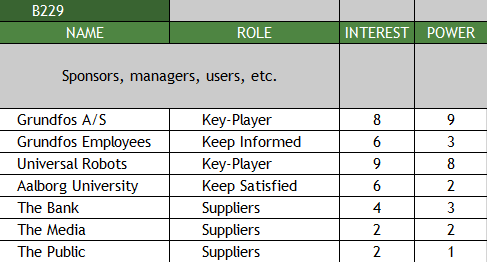
\includegraphics[scale=0.65]{StakeholderAnalysis/Stake-Ranking.PNG}
    \caption{Stakeholder Analysis} 
    \label{fig:Stakeholder-ranking} 
\end{figure}
\newpage
\begin{figure}[h]
    \centering
    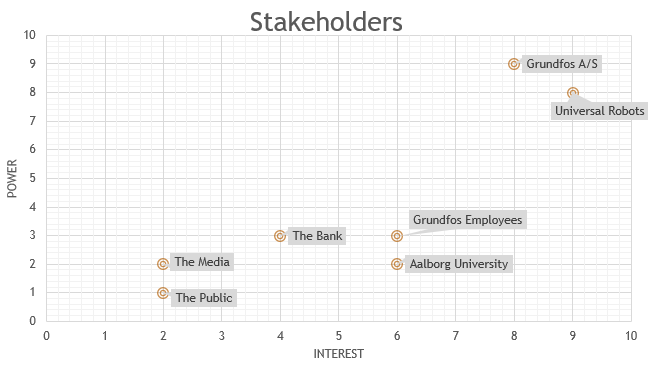
\includegraphics[scale=0.65]{StakeholderAnalysis/Stake-Graph.PNG}
    \caption{Stakeholder Analysis} 
    \label{fig:Stakeholder-graph} 
\end{figure}

\subsection{Key-Players}
The purpose of the key players, are that they have to be managed closely, thus also requiring regular meetings and updates about the progress of the design process.\\

\subsection{Keep Informed}
The purpose of this group is, that they usually have low power to influence the project, but has a great interest in it, and its impact.\\

\subsection{Suppliers}
This group usually has low power and interest in the project, as the biggest impact it can have on them is if the project is a success, they might get bigger orders for materials in the future.\\

\subsection{Keep Satisfied}
This group can have a high impact on the project, because they are sitting in places that have power to influence the direction of the project, but it is not of their primary concern, so they are designated by having high power, but low interest.\\

\section{Stakeholders}\label{ch:Stakeholders-main}

\subsection{Grundfos A/S}\label{ch:grundfosas-stake}
Grundfos A/S is a stakeholder with high interest and high power, as they are investing in the work-cell. Their interest is high, because further development of the robotic solution directly impacts the company. Development would be difficult without funding, which also gives Grundfos a lot of power. 

\subsection{Grundfos Employees}\label{ch:grundfosemp-stake}
Employees of Grundfos are stakeholders, who have a high interest, but a medium influence.\\ The reason for this is, that they have a say in whether the final solution should be implemented. Because the employees are the ones that have to collaborate with the cobot. The Employees will in some instances have to learn new skills, in order to use the robots.

\subsection{Universal Robots}\label{ch:Universalrobots-stake}
The suppliers of the robotic manipulator in this case has a high interest and a low power.\\The reason is if we should choose their manipulator over a competitors manipulator, they can then adjust the prices on the manipulator so we would choose their product in this case. 

\subsection{The Bank}\label{ch:Bank-stake}
The bank has a medium interest, and medium power in the development of a new robotic cell, the reason is that such a process is time consuming, and costly to develop, and some money has to be invested before the new design can be sold.

\subsection{The Media}\label{ch:Media-stake}
The media has a low interest, and low power to influence the development of a new robotic cell, it can have some value to the media, to write about new design technology being released to the market.

%\subsection{The Public}\label{ch:Public-stake}
%The public has low interest and low power, their interest mostly concerns, reading up on new designs and technology being made.

%\subsection{Aalborg University}\label{ch:Aau-stake}
%Aalborg University has an interest in the development of robotics from a research and information perspective. For this reason they potentially have an interest in investing in further development and improvement of a technology such as the UR. 